\begin{figure*}[t]
  \begin{center}
    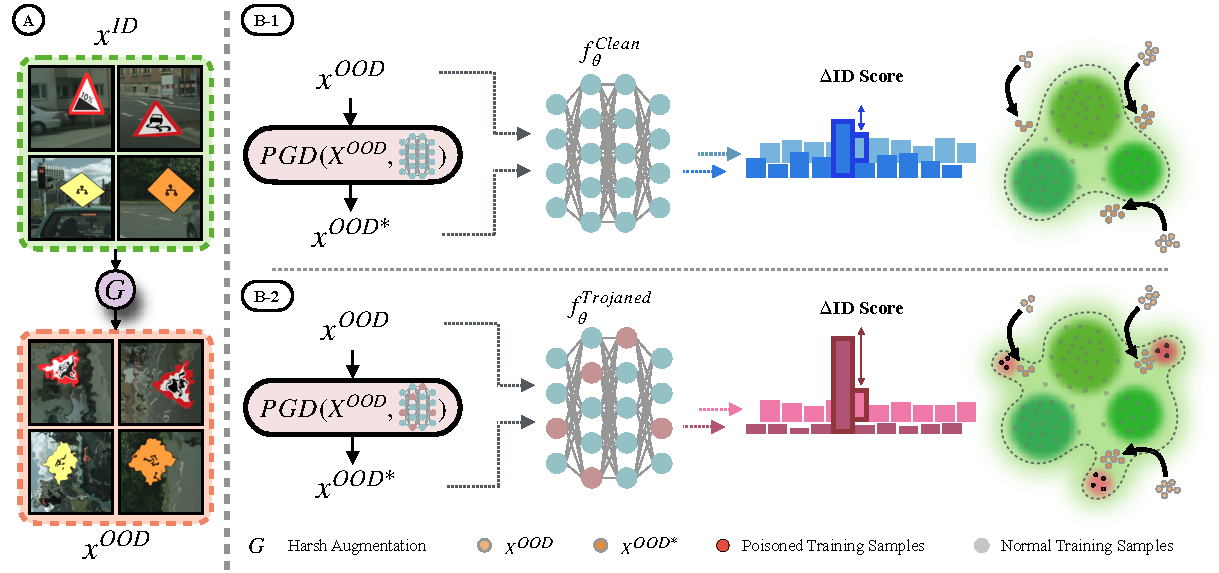
\includegraphics[width=1\linewidth]{Images/MainFigure.pdf}
    \caption{\textbf{An overview of TRODO} A) If a small portion of benign training samples was available, a module shown as \textbf{G} is used to obtain near-OOD samples. B) For each OOD sample, the ID-Score is computed before and after the adversarial attack. The difference between these scores is used as a signature to distinguish between a clean and a trojaned classifier. Performing the adversarial with not a large budget helps to discriminate between benign and trojaned classifiers 1) Lack of blind spots in the learned decision boundary of a clean model, makes it difficult to increase the ID-Score of OOD samples, resulting in small change in ID-Score. 2) For a trojaned model, $\Delta \text{\textbf{ID-Score}}$ is more discernible. This is due to the presence of blind spots, making it easier to shift OOD samples inside the decision boundary.}
\label{MainFigure}
    
    \vspace*{-6mm}

  \end{center}
\end{figure*}



% \begin{figure*}[t]
%   \begin{center}
%     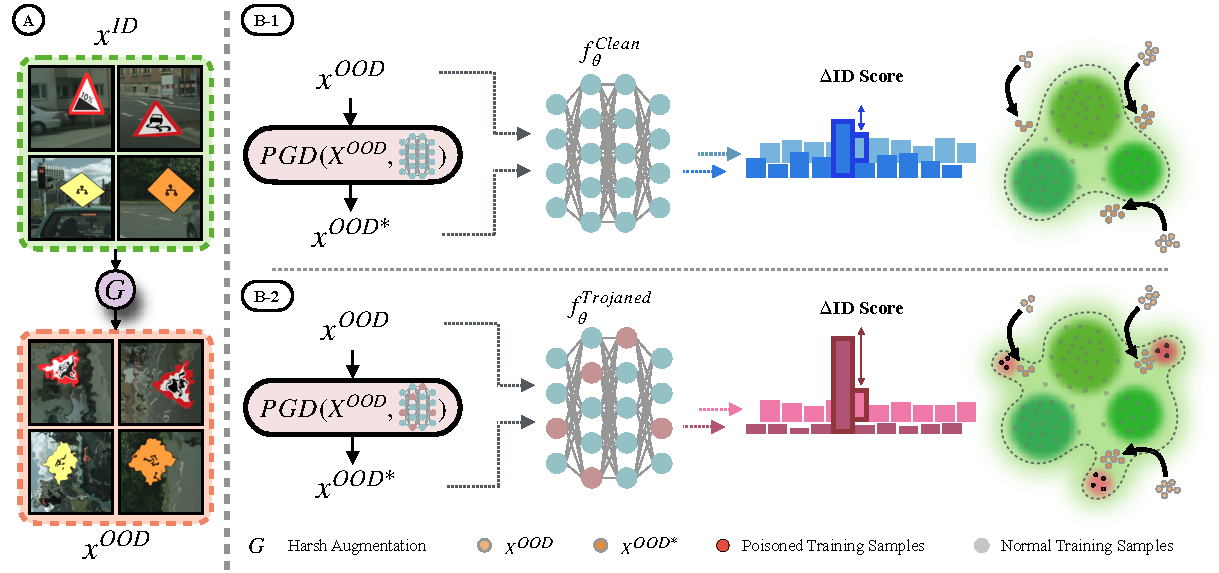
\includegraphics[width=1\linewidth, bb=0 0 600 280]{Images/MainFigure.pdf}
%     \caption{\textbf{An overview of TRODO} A) If a small portion of benign training samples was available, a module shown as \textbf{G} is used to obtain near-OOD samples. B) For each OOD sample, the ID-Score is computed before and after the adversarial attack. The difference between these scores is used as a signature to distinguish between a clean and a trojaned classifier. Performing the adversarial with not a large budget helps to discriminate between benign and trojaned classifiers 1) Lack of blind spots in the learned decision boundary of a clean model, makes it difficult to increase the ID-Score of OOD samples, resulting in small change in ID-Score. 2) For a trojaned model, $\Delta \text{\textbf{ID-Score}}$ is more discernible. This is due to the presence of blind spots, making it easier to shift OOD samples inside the decision boundary.}
%     \label{MainFigure}
%     \vspace*{-6mm}
%   \end{center}
% \end{figure*}
